\begin{figure}[H]
    \centering
    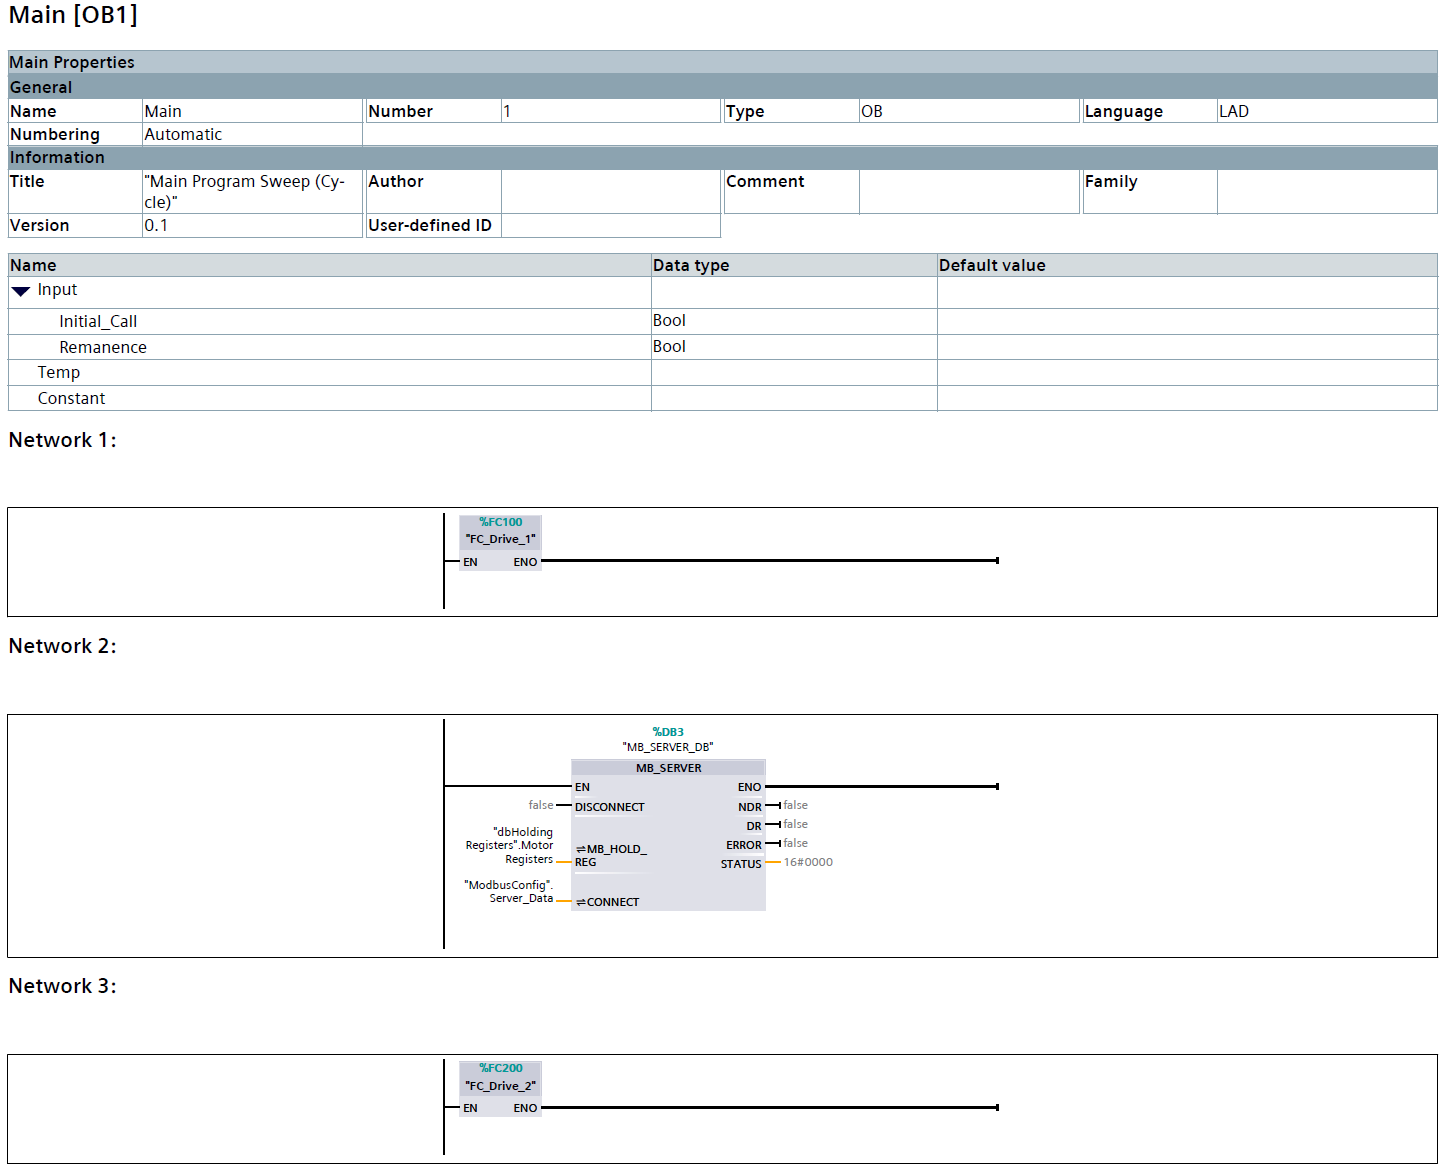
\includegraphics[width=0.5\linewidth]{FBDs/MainProgramSweep.PNG}
    \caption{Main Program Sweep cycle in the PLC}
    \label{fig:OB1}
\end{figure}


\newgeometry{scale=0.75}
\thispagestyle{empty}
{%
\begin{figure}[H]
    \centering
    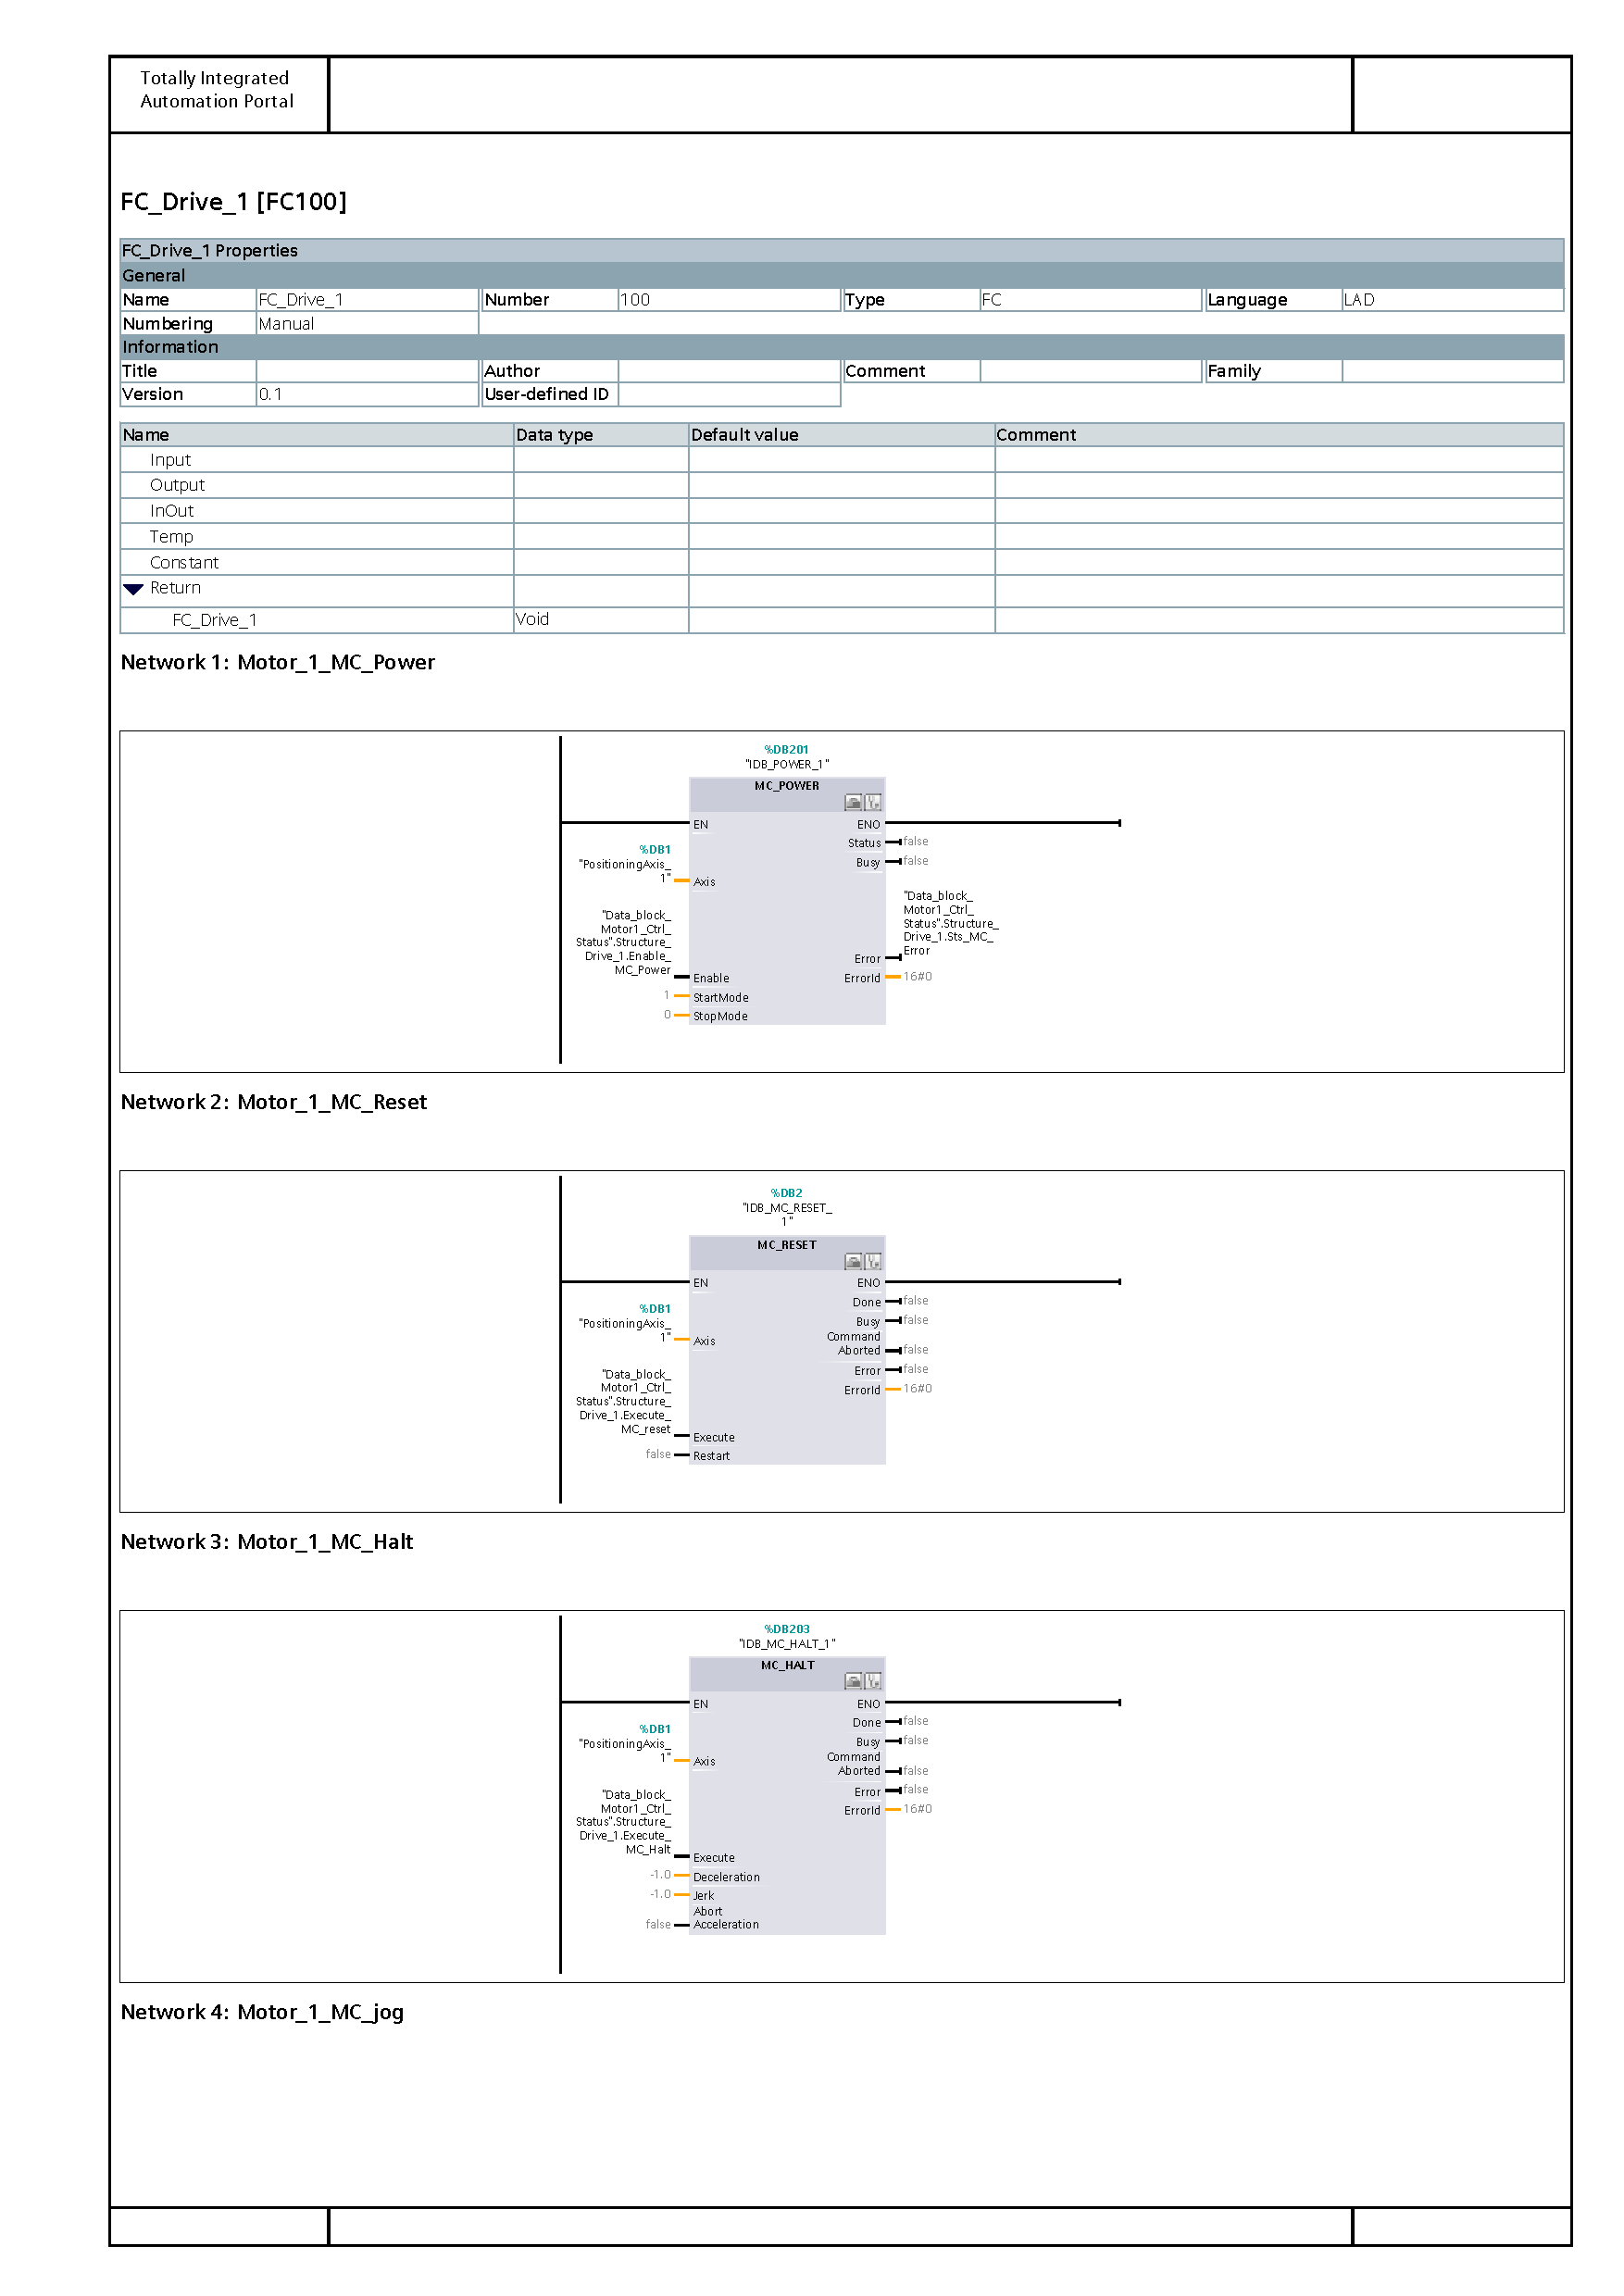
\includegraphics[page=1,scale=.5]{FBDs/FC_1.pdf}
    \caption{The function block for the control of Drive 1, the function block for Drive 2 is similar with appropriate change of variables.}
    \label{fig:FC1}
\end{figure}
  \par
}
\includepdf[pages={2-4},scale=.75]{FBDs/FC_1.pdf}
\restoregeometry

\begin{figure}[H]
    \centering
    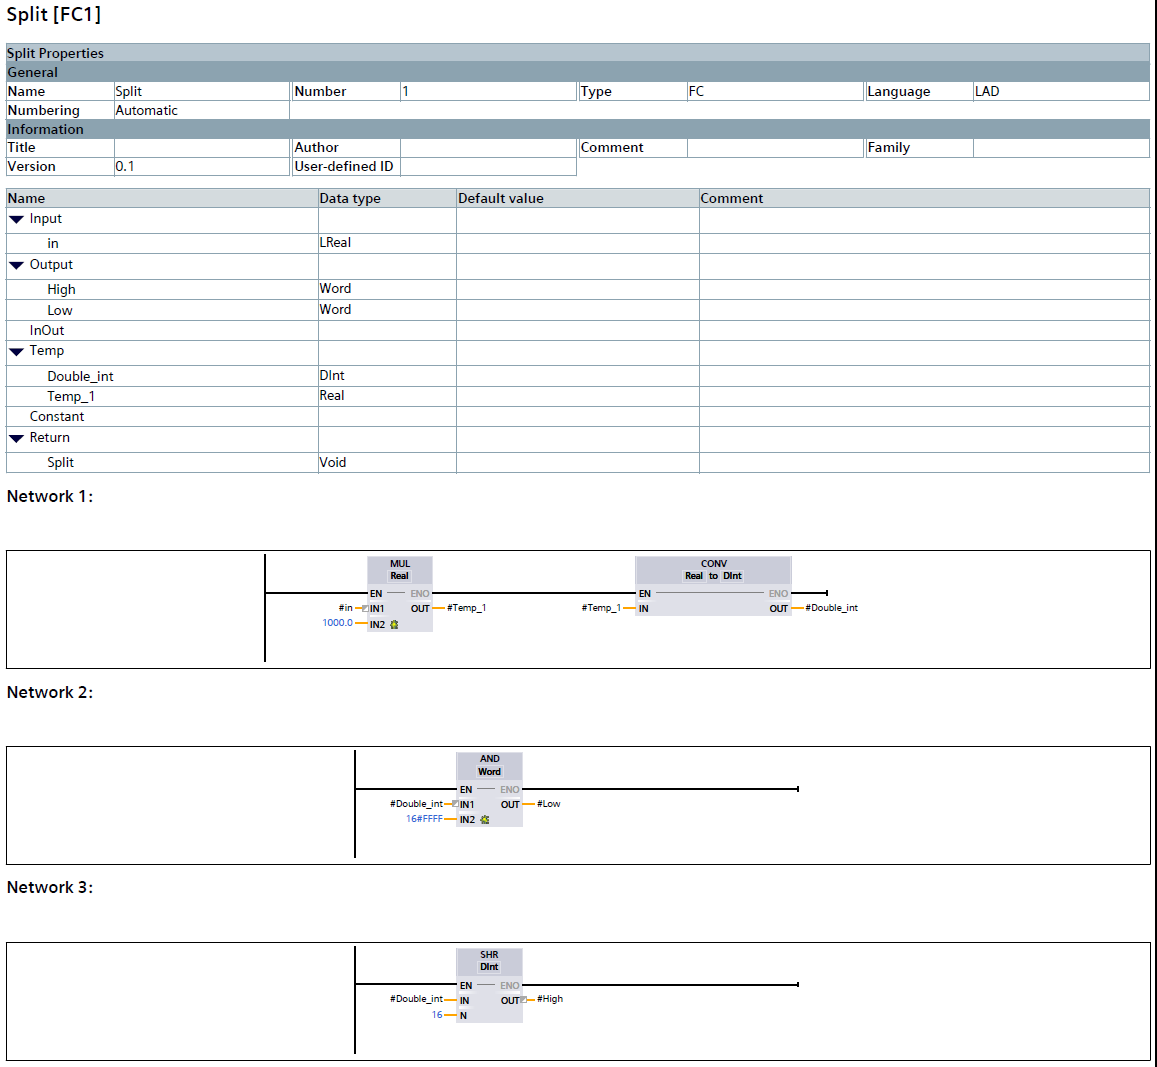
\includegraphics[width=0.5\linewidth]{FBDs/split.PNG}
    \caption{Function block for splitting a 32-bit \Gls{real} into two 16 bit \glspl{word}}
    \label{fig:split}
\end{figure}
\begin{figure}[H]
    \centering
    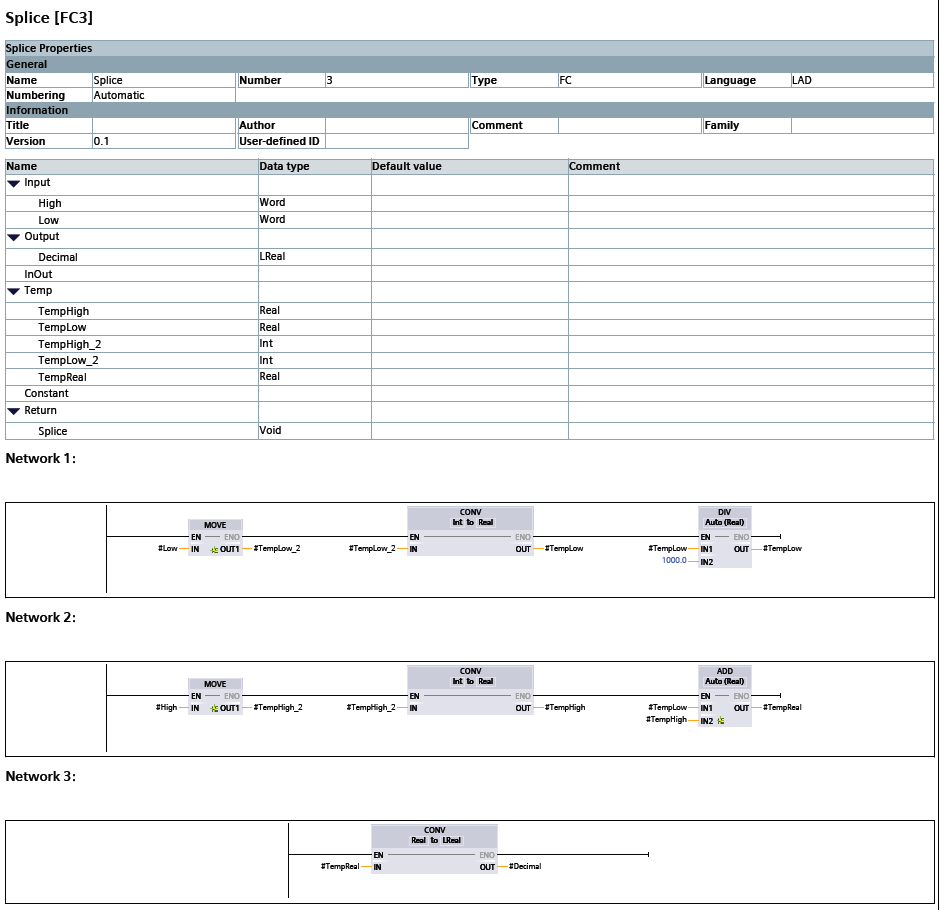
\includegraphics[width=0.5\linewidth]{FBDs/Splice.PNG}
    \caption{Function block for splicing together a 32-bit \Gls{real}(floating point value) from two 16 bit \glspl{word} before converting it to a 64 bit \Gls{lreal}.}
    \label{fig:Splice}
\end{figure}

\begin{figure}[H]
    \centering
    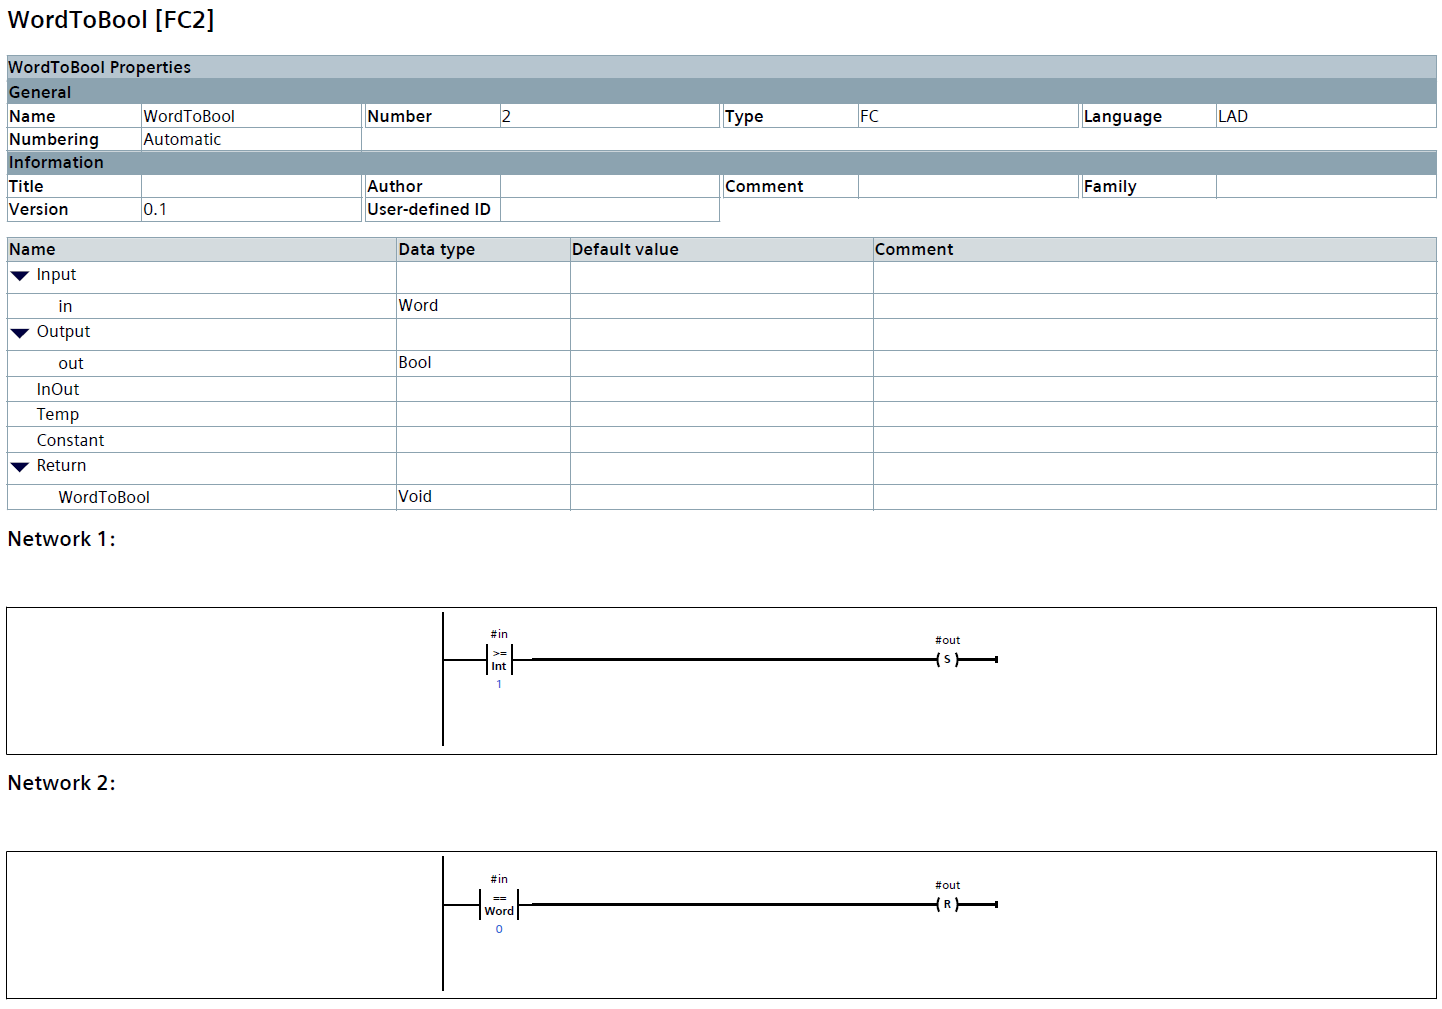
\includegraphics[width=0.5\linewidth]{FBDs/WordToBool.PNG}
    \caption{Function block for converting a 16-bit \gls{word}(which only takes the values 0 or 1) into a 1-bit \gls{bool}}
    \label{fig:WTB}
\end{figure}